%%%%%%%%%%%%%%%%%%%%%%%%%%%%%%%%%%%%%%%%%%%%%%%%%%%%%%%%%%%%%%%%%%%%%%%%%%%%%%%%
\section{The Tutorial Scenario}

%%%%%%%%%%%%%%%%%%%%%%%%%%%%%%%%%%%%%%%%%%%%%%%%%%%%%%%%%%%%%%%%%%%%%%%%%%%%%%%%
\begin{frame}
    \frametitle{Outline}
    \begin{columns}[t]
        \begin{column}{.5\textwidth}
            \tableofcontents[sections={1-9},currentsection]
        \end{column}
        \begin{column}{.5\textwidth}
            \tableofcontents[sections={10-18},currentsection]
        \end{column}
    \end{columns}
\end{frame}

%%%%%%%%%%%%%%%%%%%%%%%%%%%%%%%%%%%%%%%%%%%%%%%%%%%%%%%%%%%%%%%%%%%%%%%%%%%%%%%%
\begin{frame}
	\frametitle{What is this about?}
	\begin{question}[Questions]
		\begin{itemize}
			\item How can workflow development be started?
			\item What is a good directory layout?
			\item How does a workflow description look like?
		\end{itemize}
	\end{question}
	\begin{docs}[Objectives]
		\begin{enumerate}
			\item Introduce you to conceptualization
			\item First demonstration of directory layouts
			\item Introducing a first (very basic) workflow
		\end{enumerate}
	\end{docs}
\end{frame}

\subsection{Tasksetting}

%%%%%%%%%%%%%%%%%%%%%%%%%%%%%%%%%%%%%%%%%%%%%%%%%%%%%%%%%%%%%%%%%%%%%%%%%%%%%%%%
\begin{frame}
  \begin{figure}
    \centering
    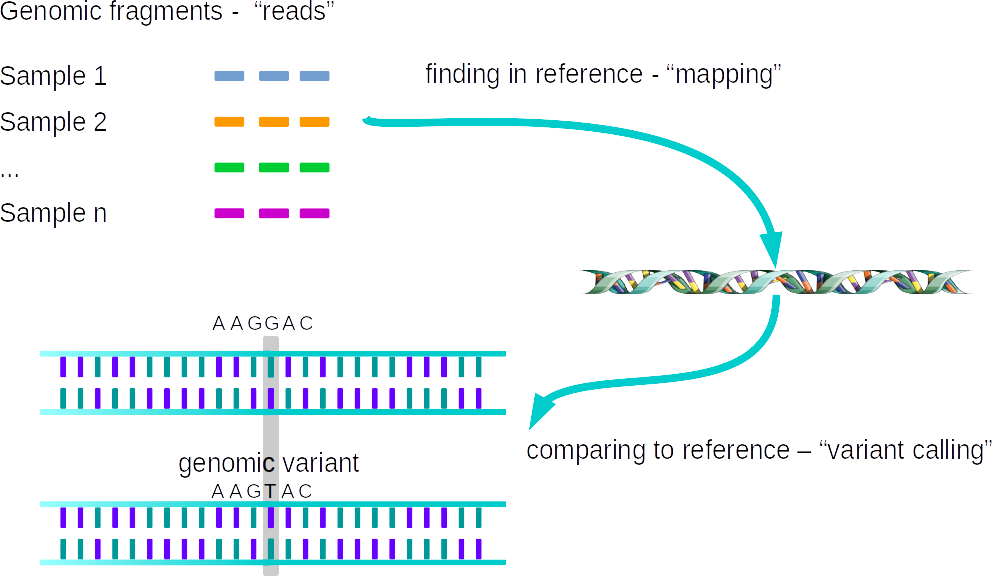
\includegraphics[width=0.95\textwidth]{biology/variant_calling_workflow.png}
  \end{figure}
\end{frame}


%TODO: Once VSC is running on logins, we should change this slide
%%%%%%%%%%%%%%%%%%%%%%%%%%%%%%%%%%%%%%%%%%%%%%%%%%%%%%%%%%%%%%%%%%%%%%%%%%%%%%%
\begin{frame}[fragile]
  \frametitle{We are almost there \ldots}
  In order to start working, we need an editor.
  \begin{itemize}[<+->]
   \item load your editor \altverb{geany} or \altverb{gedit} \emph{before} attempting to load modules in the same shell. Start it like
         \begin{lstlisting}[language=Bash, style=Shell]
$ geany & 
         \end{lstlisting}
   \item Best use a terminal multiplexer \textbf{or} multiple logins (otherwise you have to develop and execute in one shell).
  \end{itemize}
\end{frame}



